\documentclass[a4paper]{article}

\usepackage[english]{babel}
\usepackage[utf8]{inputenc}
\usepackage{amsmath}
\usepackage{graphicx}
\usepackage{color}
\usepackage{geometry}
%\usepackage[colorinlistoftodos]{todonotes}
\usepackage{array}
\usepackage{subcaption}
\newcommand{\head}[2]{\multicolumn{1}{>{\centering\arraybackslash}p{#1}}{\textbf{#2}}}
\usepackage{float}
\usepackage{amssymb}
\restylefloat{table}

%=== For listing colors =========
\usepackage{listings}
\usepackage{color}

\definecolor{codegreen}{rgb}{0,0.6,0}
\definecolor{codegray}{rgb}{0.5,0.5,0.5}
\definecolor{codepurple}{rgb}{0.58,0,0.82}
\definecolor{backcolour}{rgb}{0.95,0.95,0.92}

\lstdefinestyle{mystyle}{
	backgroundcolor=\color{backcolour},   
	commentstyle=\color{codegreen},
	keywordstyle=\color{magenta},
	numberstyle=\tiny\color{codegray},
	stringstyle=\color{codepurple},
	basicstyle=\footnotesize,
	breakatwhitespace=false,         
	breaklines=true,                 
	captionpos=b,                    
	keepspaces=true,                 
	numbers=left,                    
	numbersep=5pt,                  
	showspaces=false,                
	showstringspaces=false,
	showtabs=false,                  
	tabsize=2
}

\lstset{style=mystyle}

%===========================================

\title{Report Practical(Assignment 3)}

\author{\textbf{Team members:}\\
Fares Ben Slimane \\
Parviz Haggi \\
Mohammed Loukili \\
Jorge A. Gutierrez Ortega
}

\date{\today}

\begin{document}
\maketitle

\begin{abstract}
This report includes our solutions to the problems of the 3rd practical assignment. It consists of three sections: In Section 1 we implement the original GAN and WGAN with gradient penalty along with some experimentation. Section 2 is about the implementation and experimentation of the VAEs. The last section (3) includes experimentation and evaluation of the generative models' ability to generate realistic-looking images. In each case, our code is uploaded to the following Github repository \cite{github}
\end{abstract}

\section*{Problem 1}
\begin{enumerate}
	\item In this section, we will show the implementation of the Jensen Shannon Divergence (JSD). In order to test this function, we have implemented a neural network with the following architecture:
	\begin{itemize}
		\item 2 hidden layers, with 64 and 128 output units, respectively, and a ReLu activation function
		\item Output layer with Sigmoid activation function 
	\end{itemize}

An overview of the implementation can be seen below. The full code is available in the file \textbf{density\_estimation.py} under our github repository~\cite{github}.
	
	\lstinputlisting[language=Python]{Q1.1.py}
	
	\item In this section, we will present the implementation of the Wasserstein Distance (WD). Same neural network architecture as above was used also in this case with the exception of replacing the Sigmoid output by a linear output.
	
	The following subset of the code shows the implementation of the WD. The full code is also available in our repository~\cite{github}
	
	\lstinputlisting[language=Python]{Q1.2.py}
	
	\item Here, we have trained the above neural network with 21 combinations of $p\sim~U(0,Z)$, and $q\sim~U(\phi,Z)$, where $Z\sim~U(0,1)$ and $\phi$ is a value in the interval $[-1,1]$. The size of the distribution is 512, and the models were trained for 5000 iterations using an SGD optimizer. For every value of $\phi$ we generate a distribution and measure its distance to $p\sim~U(0,Z)$. We implement this for WD and JSD and plot their losses. 
	
	The full code is given in the file \textbf{density\_estimation.py} under our github repository~\cite{github}.
	
	The following figures show the estimated JSD for the 21 values of $\phi$ :
	\begin{figure}[H]
		\centering
		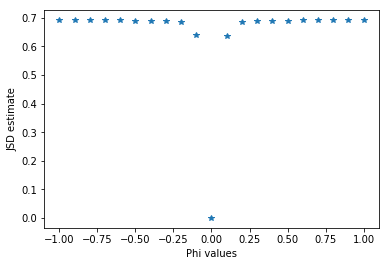
\includegraphics[scale=0.8]{jsd.png}
		\caption{JSD estimation}
		\label{fig:jsd}
	\end{figure}
	
	The estimated WD for the 21 value of $\phi$ is shown below:
	\begin{figure}[H]
		\centering
		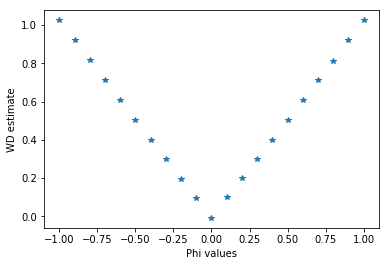
\includegraphics[scale=0.8]{wd.png}
		\caption{WD estimation}
		\label{fig:wd}
	\end{figure}

\item In this section we estimate the unknown density $f_1$ using the approximation ${f_0(x){D(x)}/(1-D(x))}$ (proven in Question 5 from the theoretical part), where $f_0$ is a known distribution (assumed 1-dimensional standard Gaussian in this question). The full code is provided in the file \textbf{density\_estimation.py} under our github repository~\cite{github}.

Using the above neural network (discriminator), we minimize the following function:
$$loss = -(torch.mean(torch.log(Dx)) + torch.mean(torch.log(1-Dy))),$$
where Dx is the feedforward of $f_1$ and Dy is the feedforward of $f_0$. 

The following figures show the discriminator's output and the estimated density:

\begin{figure}[H]
	\centering
	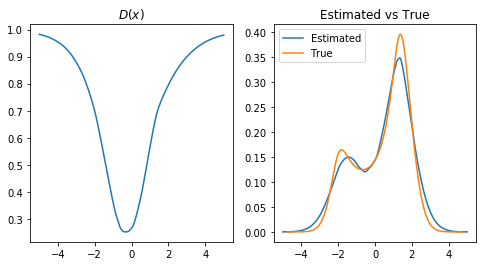
\includegraphics[scale=0.8]{disc.png}
	\caption{(left) Discriminator output (Right)Estimated $f_1$}
	\label{fig:disc}
\end{figure}



\end{enumerate}


\section{Problem 2: Implementing an RNN with Gated Recurrent Units (GRU)}

The implementation of an RNN with a gating mechanism (GRU) can be found in the gru.py script or in the models.py script. To train the model you need to execute the script ptb-ml.py.

\section*{Problem 3}
\begin{itemize}
\item[A.] {Qualitative Evaluations}\\

    \item [B.] {Quantitative Evaluations}\\
    \begin{enumerate}
        \item[1.]
       We use the provided functions to extract the representations of the images. We compute the Frechet Inception Distance by estimating the mean and covariance of the generator's/decoder's distribution. This can be seen in the following code snippet:
    \lstinputlisting[language=Python]{Q1.1.py}
        \item[2.] \\
        We sample 1000 images from our generative model and calculate the FID-score as instructed. Our results are: (ATTENTION MOHAMMED)
        \item
        \item FID
        
    \end{enumerate}
\end{itemize}





 \newpage
\begin{thebibliography}{9}
\bibitem{github} 
  Github repository for assignment 3
  \\\texttt{https://github.com/faresbs/Representation-Learning.git}

  
  
\end{thebibliography}
\end{document}